\documentclass[titlepage, 11pt]{article}
\usepackage[utf8]{inputenc}
\usepackage[margin=1in]{geometry}
\usepackage{url}
\usepackage{float}
\usepackage{graphicx}
\usepackage{hyperref}
% Define the package name here so we can change it
\newcommand{\pkgname}{\textit{ipprl\_tools}}

\title{\pkgname{} Documentation: Linkability Measures\\v1.0}
\date{July 2019}

\begin{document}

\maketitle

\tableofcontents
\section{Compatibility}
The \pkgname{} package was written using Python 3.6, but should be compatible with any version of Python 3 (Python 3.x).

\section{Required Dependencies}

\subsection{Language}
\pkgname{} requires Python 3.x to be installed prior to using the package. To check which version of Python you are using, run the following commands in your interpreter:
\begin{figure}[H]
    \centering
    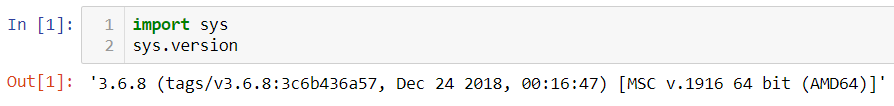
\includegraphics[width=0.9\textwidth]{imgs/Python_ver.PNG}
    \caption{Checking the installed version of Python.}
    \label{fig:pythver}
\end{figure}

\noindent To install Python, visit \url{https://www.python.org/} and download the installer for your Operating System.

\subsection{Python Package Dependencies}
The following packages are required dependencies for the \pkgname{} package. If you installed \pkgname{} through PIP, these dependencies should be installed automatically.

    \begin{itemize}
        \item \textbf{Pandas} $\geq$ v0.23
        \begin{itemize}
            \item \url{https://pandas.pydata.org}
        \end{itemize}
        \item \textbf{NumPy} $\geq$ v1.16
        \begin{itemize}
            \item \url{https://www.numpy.org}
        \end{itemize}
        \item \textbf{SciPy} $\geq$ v1.2
        \begin{itemize}
            \item \url{https://www.scipy.org}
        \end{itemize}
    \end{itemize}

\section{Optional Dependencies}
The following packages are optional dependencies for the \pkgname{} package. These dependencies will not be installed automatically when installing \pkgname{} with PIP, so they must be installed manually if needed.

\begin{itemize}
    \item \textbf{Fuzzy} $\geq$ v1.2.2
    \begin{itemize}
        \item This package is required for the Soundex corruption method. For more information about the package, visit \url{https://pypi.org/project/Fuzzy/}.
    \end{itemize}
    \item \textbf{Jupyter} $\geq$ v1.0.0
    \begin{itemize}
        \item This package is required to view and run the tutorial Jupyter notebook. For more information about Jupyter, visit \url{https://jupyter.org/}
    \end{itemize}
\end{itemize}

\section{Installation}

\subsection{PIP Method (Recommended)}
To install the package via PIP run the command:
\begin{verbatim}
    pip install git+git://github.com/cu-recordlinkage/ipprl_tools
\end{verbatim}
through a command-line interface.
\\
\\
\noindent This command will install the \pkgname{} package into your default Python environment. This command will also install the required dependencies (Pandas, NumPy, SciPy, etc) if they are not already installed. 

\subsection{GitHub Method}: 
The source code can also be cloned directly from GitHub using the following command from a command-line interface.

\begin{verbatim}
    git clone https://github.com/cu-recordlinkage/ipprl_tools
\end{verbatim}

\section{Usage}
\subsection{Importing the Package}
\label{imprt}
To use \pkgname{}, first import the \verb|metrics| submodule. 
\begin{figure}[H]
    \centering
    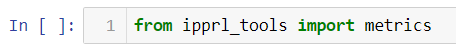
\includegraphics{imgs/ImportDoc.PNG}
    \caption{Importing \pkgname{}}
    \label{fig:my_label}
\end{figure}

\noindent This command will import all of the functions defined in the \verb|metrics| submodule. If you only need a subset of the functions, you can specify the exact functions to import as well:

\begin{figure}[H]
    \centering
    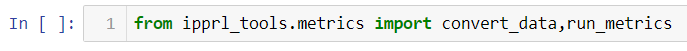
\includegraphics{imgs/ImportDocFunctions.PNG}
    \caption{Importing specific functions}
    \label{fig:my_label}
\end{figure}

\subsection{Data Prerequisites}
\label{data_prereqs}
The linkability metric functions expect that data will be contained in a Pandas DataFrame. To read in a file using Pandas, first call the appropriate read function. In our case we are reading CSV data, so we use \textit{pandas.read\_csv()}, but alternative functions are available for other types of data.

\noindent For additional ways to import data using Pandas, refer to the Pandas Documentation here:
\\
\\
\href{https://pandas.pydata.org/pandas-docs/stable/user_guide/io.html}{Pandas Documentation: IO}
\\

\begin{figure}[H]
    \centering
    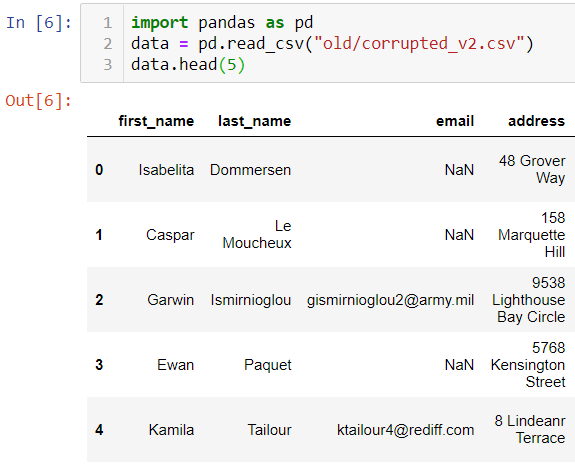
\includegraphics{imgs/PandasRead.png}
    \caption{Reading in a CSV file with Pandas}
    \label{fig:my_label}
\end{figure}

The linkability metric functions provided in \pkgname{} are designed to operate on Pandas DataFrames, but in order for them to work correctly, we must first ensure that the DataFrame is in the correct format.
\\
\\
\noindent By default, Pandas will attempt to parse columns of your input file differently, depending on the type of data in the column.
\begin{figure}[H]
    \centering
    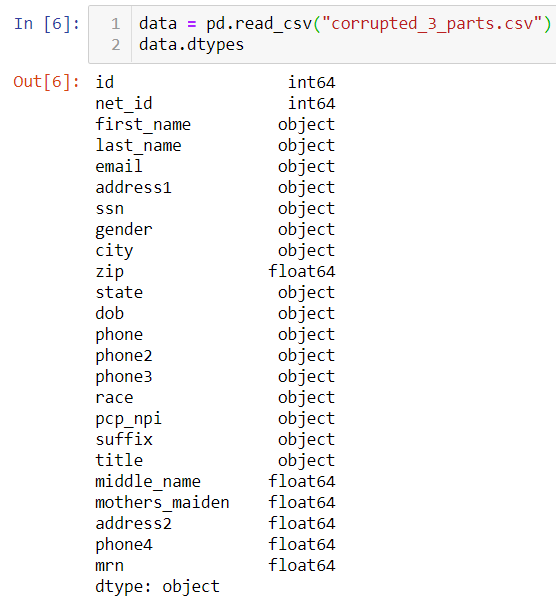
\includegraphics[width=0.6\textwidth]{imgs/DataTypes.PNG}
    \caption{Data types of each column, after reading data from a CSV file.}
    \label{fig:my_label}
\end{figure}

\noindent In this case, Pandas has parsed some of the numerical columns (\textit{id}, \textit{zip}, etc.) as different data types. In order for the linkability metrics to work, we first need to convert all columns in the DataFrame to the \textit{string} data type. We also need to ensure that missing data is handled in the correct way. All linkability metrics treat the empty string ("") as a missing value.
\\
\\
\noindent In order to make this process easy, \pkgname{} contains a function called \textit{convert\_data()} (\ref{cnvrt_data}), which can be used to automatically convert a DataFrame to the correct format. 
To use, import \textit{convert\_data} from the \pkgname\textit{.metrics} submodule, then call it on your DataFrame.

\begin{figure}[H]
    \centering
    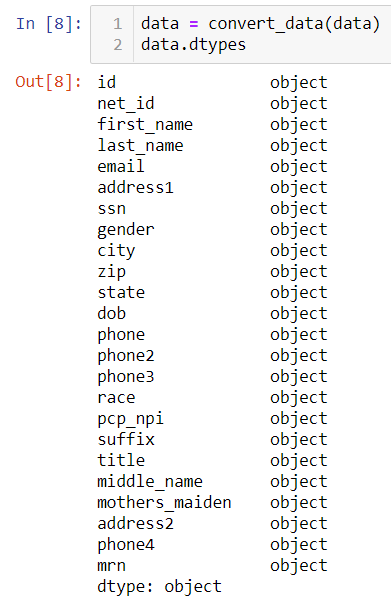
\includegraphics[width=0.4\textwidth]{imgs/DtypesConverted.PNG}
    \caption{Example of calling \textit{convert\_data()} and viewing the result.}
    \label{fig:my_label}
\end{figure}

\noindent In the above figure, we call \textit{metrics.convert\_data()} on our DataFrame, and view the data types of the output. We can see that the DataFrame was converted correctly, as every column is now of \textit{type(object)}.
\\
\subsection{Computing Metrics}
\subsubsection{Calling Individual Functions}
To call a linkability metric on a DataFrame, first ensure that you've imported the function by following the instructions in Section \ref{imprt}.

We can call an individual function on every column in the DataFrame, or specify some subset of the columns to use. 

\begin{figure}[H]
    \centering
    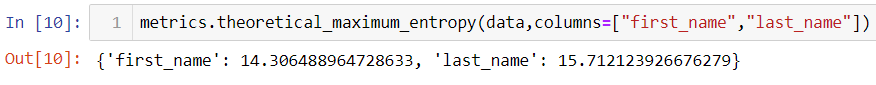
\includegraphics[width=0.8\textwidth]{imgs/ColumnSubset.PNG}
    \caption{Example of calling a linkability metric by manually specifying the columns to operate on.}
    \label{fig:column_subset}
\end{figure}

\begin{figure}[H]
    \centering
    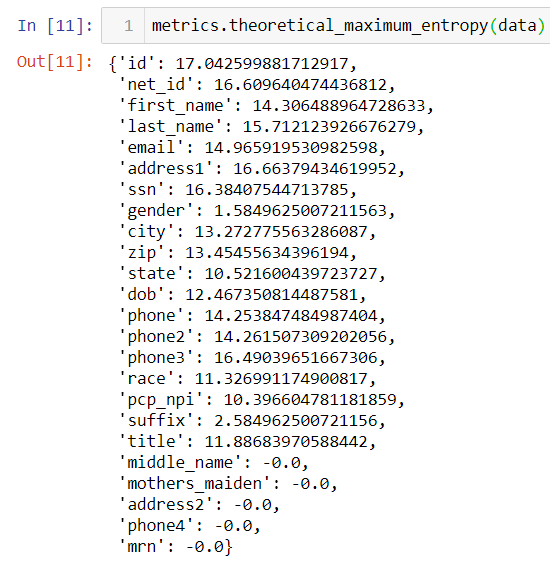
\includegraphics[width=0.6\textwidth]{imgs/AllColumns.PNG}
    \caption{Example of calling a linkability metric by using the default column argument (all columns)}
    \label{fig:all_columns}
\end{figure}

\noindent In either case, the output of each linkability metric is a Python \textit{dict} object, which has keys corresponding to the names of the selected columns, and values corresponding to the calculated linkability metric.

\subsubsection{Using \textit{run\_metrics()}}
Although each metric can be run individually, \pkgname{} also provides a helper function to run all of the metrics at once, and provide a formatted output DataFrame.
\\
\noindent To use this function, import \textit{run\_metrics} from the \textit{ipprl\_tools.metrics} submodule, and call it on your DataFrame.

\begin{figure}[H]
    \centering
    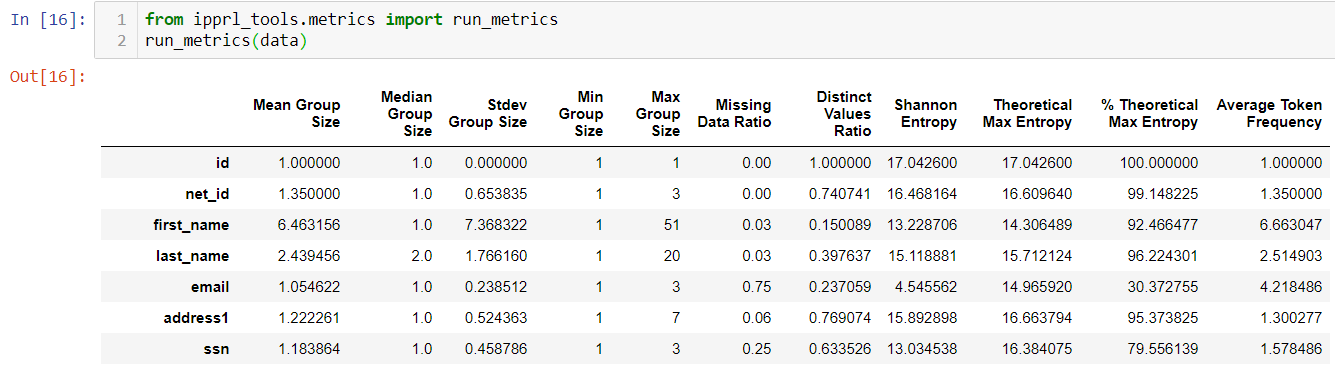
\includegraphics[width=\textwidth]{imgs/RunMetricsExample.PNG}
    \caption{Example of importing and using the \textit{run\_metrics} function.}
    \label{fig:run_metrics}
\end{figure}

\noindent The output of the function is a formatted Pandas DataFrame, where each column corresponds to a linkability metrics, and the rows are the columns from your original DataFrame.

\section{Function Documentation}


%% Declaring some documentation macros here

%% Generic macro to make a formatted function description
\newcommand{\parmdesc}[2]{\textit{#1} - #2}

%% Description for the data parameter.
\newcommand{\docdata}{\parmdesc{data}{The Pandas DataFrame to be modified. Please ensure that your data is in the correct format (as specified in Section \ref{data_prereqs}) before passing as an argument.}}

%% Description for the columns parameter
\newcommand{\doccols}{\parmdesc{columns}{An optional list of columns to operate on. These columns should correspond to column names in the DataFrame that you would like to calculate metrics for. The default argument (\textit{columns=None}) will calculate metrics for each column in \textit{data}.}}

% Description for the return value dictionary
\newcommand{\docreturn}[1]{\parmdesc{values}{A dictionary containing a key/value mapping of \textit{column\_name} $\rightarrow$ \textit{#1} for each column specified in \textit{columns}.}} 

\subsection{Linkability Metrics}

\subsubsection{\textit{missing\_data\_ratio(data, columns=None)}}

This function calculates the Missing Data Ratio, or MDR for each of the specified columns. The Missing Data Ratio is defined as: 
\begin{equation}
    MDR_i = \frac{Number\, of\, records\, with\, missing\, value\, in\, Variable_i} {Total\, number\, of\, records\, in\, Variable_i}
\end{equation}
This metric can be used to determine what fraction of the columns values are usable for linkage.
\\
\\
\textbf{Parameters:}
\begin{itemize}
    \item \docdata
    \item \doccols
\end{itemize}
\textbf{Return Value:}
\begin{itemize}
    \item \docreturn{mdr\_value}
\end{itemize}


\subsubsection{\textit{distinct\_values\_ratio(data, columns=None)}}
This function calculates the Distinct Values Ratio (DVR), which is defined as:
\begin{equation}
    DVR_i = \frac{Number\, of\, distinct\, values\, for\, Variable_i} {Number\, of\, records\, in\, Variable_i}
\end{equation}
This metric can be used to determine how many unique values a variable/column has, relative to its size. A high DVR indicates that there are a large number of distinct values in the column, whereas a low DVR indicates that there are fewer distinct values.
\\
\\
\textbf{Parameters:}
\begin{itemize}
    \item \docdata
    \item \doccols
\end{itemize}
\textbf{Return Value:}
\begin{itemize}
    \item \docreturn{dvr\_value}
\end{itemize}

\subsubsection{\textit{group\_size(data, columns=None)}}
\label{grp_size}
This function calculates and returns the Group Sizes for each distinct value in each \textit{column}. Group Size is defined as:
\begin{equation}
    GS_i,_j = {Number\, of\, rows\, for\, Variable_i, Value_j}
\end{equation}
This function is used to calculate \textit{agg\_group\_size} (\ref{agrp_size}), but may also be called by the user. 
\\
\textbf{Parameters:}
\begin{itemize}
    \item \docdata
    \item \doccols
\end{itemize}
\textbf{Return Value:}
\begin{itemize}
    \item \parmdesc{values (\textit{dict})}{For each column name in \textit{columns}, returns a Counter object holding key/value mappings of \textit{distinct\_value} $\rightarrow$ \textit{num\_of\_occurrences}} 
\end{itemize}

\subsubsection{\textit{agg\_group\_size(data, agg\_func = np.mean, columns=None)}}
\label{agrp_size}
This function calculates the aggregate group size for each column specified in \textit{columns}, based on an arbitrary function \textit{agg\_func}. 
The function calls \textit{group\_size()} (\ref{grp_size}), and uses \textit{agg\_func} to reduce the results to a scalar value for each column. 
\\
\textbf{Parameters:}
\begin{itemize}
    \item \docdata
    \item \parmdesc{agg\_func}{This is an arbitrary reduction function which accepts a list of values, and returns a scalar. Some examples of compatible reduction/aggregation functions are: \textit{numpy.amin}, \textit{numpy.amax}, \textit{numpy.mean}, and \textit{numpy.std}. The default argument (\textit{agg\_func = np.mean}) will pass NumPy's mean function to compute the mean group size for each column name specified in \textit{columns}. }
    \item \doccols
\end{itemize}
\textbf{Return Value:}
\begin{itemize}
    \item \docreturn{agg\_group\_size\_val}
\end{itemize}

\subsubsection{\textit{shannon\_entropy(data, columns=None)}}
\label{entr}
This function calculates the Shannon Entropy for each column name specified in \textit{columns}. Shannon Entropy is defined as:
\begin{equation}
    H_x = -\sum_{i=1}^{N}P(i) \, log_2 \,P(i)
\end{equation}
This metric is useful for determining the amount of information containing in a column. Typically, columns with large numbers of evenly distributed unique values will have higher values for Shannon Entropy.
\\
\\
\textbf{Parameters:}
\begin{itemize}
    \item \docdata
    \item \doccols
\end{itemize}
\textbf{Return Value:}
\begin{itemize}
    \item \docreturn{shannon\_entropy}
\end{itemize}

\subsubsection{\textit{theoretical\_maximum\_entropy(data, columns=None)}}
\label{tentr}
This function calculates the Theoretical Maximum Entropy (TME) for a column, given its current number of distinct values. The formal definition for Theoretical Maximum Entropy is:
\begin{equation}
    TME_x= -log_2(\frac{1}{N})
\end{equation}
where \textit{N} is the number of distinct values in the column. 
\\
\\
\textbf{Parameters:}
\begin{itemize}
    \item \docdata
    \item \doccols
\end{itemize}
\textbf{Return Value:}
\begin{itemize}
    \item \docreturn{theo\_max\_entropy}
\end{itemize}

\subsubsection{\textit{percent\_theoretical\_maximum\_entropy(data, columns=None)}}

This function will calculate the Percent of Theoretical Maximum Entropy (PTME) for each column name specified in \textit{columns}. The Percent of Theoretical Maximum Entropy is defined as:
\begin{equation}
    PTME_x = \frac{H_x}{TME_x}*100
\end{equation}
Where $H_x$ and $TME_x$ are the Shannon Entropy and Theoretical Maximum Entropy of the column, respectively. This function will call \textit{theoretical\_maximum\_entropy()} (\ref{entr}) and\\ \textit{percent\_theoretical\_maximum\_entropy} (\ref{tentr}) in order to calculate the result.
\\
\\
\textbf{Parameters:}
\begin{itemize}
    \item \docdata
    \item \doccols
\end{itemize}
\textbf{Return Value:}
\begin{itemize}
    \item \docreturn{pct\_theo\_max\_entropy}
\end{itemize}

\subsubsection{\textit{average\_token\_frequency(data, columns=None)}}

This function will calculate the Average Token Frequency (ATF) for each column name specified in \textit{columns}. The Average Token Frequency is defined as:
\begin{equation}
    ATF = \frac{|V|}{N}
\end{equation}
Where $|V|$ is the size of the column, and $N$ is the number of unique values in the column.
\\
\\
\textbf{Parameters:}
\begin{itemize}
    \item \docdata
    \item \doccols
\end{itemize}
\textbf{Return Value:}
\begin{itemize}
    \item \docreturn{avg\_tok\_freq}
\end{itemize}

\subsection{Utilities}
The utilities functions are a set of functions provided alongside the Linkability Metric functions in order to perform common tasks associated with calculating linkability metrics on a dataset.

\subsubsection{\textit{convert\_data(data)}}
\label{cnvrt_data}
This function will convert the Pandas DataFrame \textit{data} into a format suitable for calculating linkability metrics. The function will convert \textit{data} to a DataFrame of string objects, automatically converting $NaN$ values to the empty string ("").
\\
\\
\textbf{Parameters:}
\begin{itemize}
    \item \parmdesc{data}{The Pandas DataFrame to be converted. If your DataFrame contains columns that are not of \textit{type(str)}, or a value for $NaN$ that is not the empty string (""), you will need to call this function to convert your DataFrame before running any of the linkage metrics.}
\end{itemize}
\textbf{Return Value:}
\begin{itemize}
    \item \parmdesc{data}{A version of the input DataFrame that has been converted to \textit{type(str)}, and had all $NaN$ values replaced with the empty string.}
\end{itemize}

\subsubsection{\textit{run\_metrics(data)}}

This function is a helper function to automatically calculate all linkability metrics on all columns in \textit{data}. The output will be collected and formatted into a Pandas DataFrame.
\\
\\
\textbf{Parameters:}
\begin{itemize}
    \item \docdata
\end{itemize}
\textbf{Return Value:}
\begin{itemize}
    \item \parmdesc{metrics\_df}{A Pandas DataFrame containing the values of every linkability metric calculated on every column in \textit{data}. The columns of the DataFrame corrsepond to the linkability metrics, and the rows correspond to the names of the columns in \textit{data.columns}.}
\end{itemize}

\end{document}
